% !TEX root = ../main.tex
\section{Q11: Boundaries of the Firm -- vertikal integrasjon, outsourcing og market power}\label{q:11}

\begin{quote}
\emph{Med udgangspunkt i termerne Boundaries of the Firm, regnskabsmæssig kontra økonomisk profit, ejerskab af produktionsfaktorer bedes begreberne vertikal integration og outsourcing præsenteret og diskuteret med hensyn til fordele og ulemper. Redegør i forlængelse heraf for modellen omhandlende vertical integration som instrument til at opnå market power.}
\end{quote}

\subsection*{Svar (kort)}
Firmaets grenser (\emph{Boundaries of the Firm}) bestemmes av avveiningen mellom transaksjonskostnader i markedet og byråkratikostnader internt (Coase 1937, Williamson 1985). Vertikal integrasjon lønner seg når spesifikke aktiva, usikkerhet og hold-up gjør markedskontrakter dyrere enn intern styring -- men den bringer egne \thref{agency-costs}{agency costs}. Sondringen mellom regnskapsmessig og økonomisk profitt avgjør om en aktivitet reelt skaper verdi innenfor firmaets grenser. Modellen for market power viser at vertikal integrasjon kan brukes strategisk til å stenge ute konkurrenter ved å kontrollere et kritisk input (foreclosure). [SLIDE]

\subsection*{Relevante teorier (kort)}

\paragraph{\thref{boundaries-of-the-firm}{Boundaries of the Firm}\quad\SOne}
Coase: firmaet erstatter markedstransaksjoner med hierarki når transaksjonskostnader er høye. Williamson: make-or-buy avhenger av asset specificity, usikkerhet og frekvens. Eierskap av produktionsfaktorer gir \emph{residuelle beslutningsrettigheter} i situasjoner kontrakten ikke dekker (Grossman--Hart--Moore). Firmaets grense trekkes der marginal intern organiseringskostnad = marginal transaksjonskostnad. [SLIDE]

\paragraph{\thref{accounting-vs-economic-profit}{Regnskabsmæssig vs.\ økonomisk profit}\quad\STwo}
Regnskapsprofitt = inntekter $-$ eksplisitte kostnader. Økonomisk profitt = inntekter $-$ alle kostnader inkl.\ \emph{opportunity cost}. En internt utført aktivitet kan vise positiv regnskapsprofitt men negativ økonomisk profitt -- da bør den outsources. BSZ Table 8.1 (BP gasoline) illustrerer: regnskapsprofitt \$1{,}2M vs.\ økonomisk profitt $-$\$400k. Kobling til \thref{responsibility-centers}{investment centers} og EVA. [SLIDE]

\paragraph{\thref{vertical-integration-outsourcing}{Vertikal integrasjon og outsourcing}\quad\SOne/\SThree}
Outsourcing gir markedsdisiplin, spesialisering, fleksibilitet og sterkere insentiver (leverandør er residual claimant). Integrasjon gir kontroll, koordinasjon, beskyttelse av IP, og eliminerer kontraktproblemer (\thref{hold-up-problem}{hold-up}, \thref{free-rider-problem}{free-riding}, \thref{double-markup-problem}{double markup}). Valget er en trade-off mellom transaksjonskostnader og byråkratikostnader. Se Q12 for de tre kontraktproblemene i dybden. [SLIDE]

\paragraph{\thref{vertical-integration-market-power}{VI som instrument til market power}\quad\SOne}
BSZ kap.\ 19-modellen: oppstrøms monopolist $U$ integrerer fremover til $D_1$ og kontrollerer dermed tilgang til input for rivaler $D_2, D_3$. $U$--$D_1$ kan foreta \emph{foreclosure} (nekte/overprise input) eller \emph{raising rivals' costs}. Sluttforbrukerpris stiger, kvantum synker. Forutsetter oppstrøms monopol og manglende regulering. Chicago School-kritikken: monopolisten kan allerede ekstrahere surplus via input-pris -- VI tilfører da ikke ny markedsmakt. [SLIDE/BOK]

\subsection*{Illustrasjoner fra forelesning}

\begin{figure}[h]
  \centering
  
\includegraphics[width=0.6\linewidth]{BSZ_kap_8_2026/by_slide/slide_002/BSZ_kap_8_2026_slide_002_asset_01_image1.jpeg}
  \caption{Firmaets grenser: strategiske valg om hva som skal gjøres internt (make) vs.\ eksternt (buy) -- Boundaries of the Firm. (BSZ kap.\ 8, slide 2) [SLIDE]}
\end{figure}

\subsection*{Illustrasjon -- accounting vs.\ economic profit}

\begin{figure}[h]
  \centering
  
\includegraphics[width=0.7\linewidth]{BSZ_kap_8_2026/by_slide/slide_011/BSZ_kap_8_2026_slide_011_asset_01_image6.png}
  \caption{BSZ Table 8.1: BP Retail Gasoline Stations -- regnskapsmessig vs.\ økonomisk profitt. Ved \$3{,}60/gallon er accounting profit positiv men economic profit negativ. Aktiviteten bør outsources. [SLIDE -- BSZ kap.\ 8]}
\end{figure}

\subsection*{Illustrasjon -- market power-modellen (TikZ)}

\begin{figure}[h]
\centering
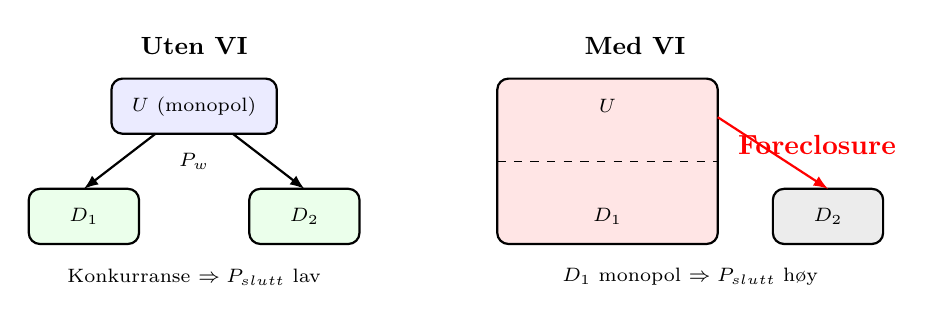
\begin{tikzpicture}[>=latex, scale=0.7, every node/.style={font=\scriptsize}]
  % Uten VI
  \node[font=\small\bfseries] at (3, 5.8) {Uten VI};
  \draw[thick, rounded corners, fill=blue!8] (1.5,4.2) rectangle (4.5,5.2);
  \node at (3,4.7) {$U$ (monopol)};
  \draw[thick, rounded corners, fill=green!8] (0,2.2) rectangle (2,3.2);
  \node at (1,2.7) {$D_1$};
  \draw[thick, rounded corners, fill=green!8] (4,2.2) rectangle (6,3.2);
  \node at (5,2.7) {$D_2$};
  \draw[->, thick] (2.3,4.2) -- (1,3.2);
  \draw[->, thick] (3.7,4.2) -- (5,3.2);
  \node at (3,3.7) {$P_w$};
  \node at (3,1.6) {Konkurranse $\Rightarrow P_{\text{slutt}}$ lav};
  % Med VI
  \begin{scope}[xshift=8cm]
  \node[font=\small\bfseries] at (3, 5.8) {Med VI};
  \draw[thick, rounded corners, fill=red!10] (0.5,2.2) rectangle (4.5,5.2);
  \node at (2.5,4.7) {$U$};
  \node at (2.5,2.7) {$D_1$};
  \draw[dashed] (0.5,3.7) -- (4.5,3.7);
  \draw[thick, rounded corners, fill=gray!15] (5.5,2.2) rectangle (7.5,3.2);
  \node at (6.5,2.7) {$D_2$};
  \draw[->, thick, red] (4.5,4.5) -- (6.5,3.2);
  \node[red, font=\bfseries] at (6.3,4.0) {Foreclosure};
  \node at (4,1.6) {$D_1$ monopol $\Rightarrow P_{\text{slutt}}$ høy};
  \end{scope}
\end{tikzpicture}
\caption{Vertikal integrasjon for market power: $U$--$D_1$ integrerer og stenger ute $D_2$ via foreclosure. [SLIDE/BOK -- BSZ kap.\ 19]}
\end{figure}

\subsection*{Real-world eksempler}

\textbf{Eks.~1 -- De Beers (diamantindustrien).}\quad [EKS]
De Beers kontrollerte historisk $\sim$80\% av verdens rådiamantproduksjon (oppstrøms monopol) og integrerte nedstrøms via Central Selling Organisation for distribusjon. Uavhengige slipere og forhandlere ble tvunget til å kjøpe via De Beers eller ble stengt ute (\emph{foreclosure}). Resultatet var kontrollert tilbud og kunstig høye diamantpriser i tiår. Modellen for VI og market power beskriver mekanismen presist.

\textbf{Eks.~2 -- Mærsk/APM Terminals, sammenligning.}\quad [EKS/CASE]
Mærsk integrerte nedstrøms i terminal-operasjoner (APM Terminals) -- men primærmotivet var \emph{effektivitet} (sikre havnekapasitet, redusere holdetid) snarere enn foreclosure av rivaler. EU-kommisjonen har vurdert om integrasjonen gir Mærsk urimelig konkurransefordel i rederibransjen, men godkjent fusjoner under vilkår om tredjepartstilgang. Sammenligningen med De Beers viser at VI kan ha ulike motiver: effektivitet (Mærsk) vs.\ rent-seeking (De Beers). Grensen er sentral for konkurranserett.

\subsection*{Kobling til Mærsk Power-to-X}
PtX illustrerer make-or-buy-beslutningen konkret: skal Mærsk produsere grønt hydrogen selv (integrere bakover i elektrolyse) eller kjøpe på markedet? Argumenter for integrasjon: spesifikt aktivum (elektrolyseanlegg tilpasset Mærsks spesifikasjon), usikkerhet om hydrogenmarkedets modenhet, beskyttelse av teknologisk forsprang. Argumenter for outsourcing: manglende kjernekompetanse i energiproduksjon, skalafordeler hos dedikerte energiselskaper. Økonomisk profitt-analysen er avgjørende: regnskapet kan vise positiv margin på intern produksjon, men alternativkostnaden (kapital bundet i elektrolyseanlegg i stedet for i rederidrift) kan gjøre $\pi_{\text{economic}}<0$. [CASE]

\subsection*{Fallgruber}
\begin{itemize}\setlength{\itemsep}{2pt}
\item Glemme å definere \emph{economic} vs.\ \emph{accounting} profit eksplisitt -- spørsmålet nevner det direkte.
\item Bare ramse opp fordeler/ulemper uten å forankre i transaksjonskostnadsteori (Coase/Williamson).
\item Forveksle Q11 med Q12: Q11 handler om \emph{Boundaries of the Firm} og \emph{market power}; Q12 handler om de tre \emph{kontraktproblemene} (hold-up, free-rider, double markup).
\item Glemme modellen for market power -- spørsmålet ber eksplisitt om den.
\item Ignorere Chicago School-kritikken av market power-argumentet.
\item Tegne market power-modellen feil: det er oppstrøms monopol + nedstrøms foreclosure, ikke omvendt.
\end{itemize}

\subsection*{Håndskrivbar disposisjon (15-min forberedelse)}
\begin{itemize}\setlength{\itemsep}{2pt}
\item \textbf{Tese:} Firmaets grenser bestemt av transaksjonskost vs.\ byråkratikost; VI lønner seg ved spesifikke aktiva, usikkerhet, markedsmakt.
\item \thref{boundaries-of-the-firm}{Boundaries of the Firm}: Coase, Williamson, eierskap = residuell kontroll (GHM).
\item \thref{accounting-vs-economic-profit}{Acc.\ vs.\ econ.\ profit}: $\pi_{\text{econ}} = R - C_{\text{exp}} - C_{\text{opp}}$. BP-eksempel Table 8.1.
\item \textbf{Fordeler outsourcing:} markedsdisiplin, skala, fleksibilitet, sterkere insentiver.
\item \textbf{Fordeler VI:} hold-up eliminert, kontroll, koordinasjon, IP-beskyttelse, market power.
\item \thref{vertical-integration-market-power}{Market power-modell}: $U$ monopol $\to$ integrerer $D_1$ $\to$ foreclosure av $D_2$. Figur.
\item Chicago-kritikk: VI tilfører ikke ny markedsmakt hvis $U$ allerede kan ekstrahere via inputpris.
\item Eks.\ 1: De Beers (foreclosure). Eks.\ 2: Mærsk/APM Terminals (effektivitet vs.\ foreclosure).
\item Case: Mærsk PtX -- make-or-buy for elektrolyse; econ.\ profit-analyse.
\item Søyle: \SOne\ (eierskap, beslutningsrett) + \STwo\ (profittbegrep).
\end{itemize}
